\documentclass[10 pt,usenames,dvipsnames, oneside]{article}
\usepackage{../../../modelo-ensino-medio}



\begin{document}

\begin{center}
  \begin{minipage}[l]{3cm}
\includegraphics[width=2cm]{logo}    
\end{minipage}\hfill
\begin{minipage}[r]{.8\textwidth}
 {\Large \scshape Atividade: Ação promocional}  
\end{minipage}
\end{center}
\vspace{.2cm}

\ifdefined\prof
\begin{objetivos}
\item \textbf{LAF1} Compreender função como uma relação de dependência entre duas variáveis, as ideias de domínio, contradomínio e imagem, e suas representações algébricas e gráficas e utilizá-las para analisar, interpretar e resolver problemas em contextos diversos, inclusive fenômenos naturais, sociais e de outras áreas.
\end{objetivos}

\begin{goals}
\begin{enumerate}

\item[OE1] Reconhecer vantagens da representação gráfica. Na questão, mais especificamente, em detrimento da representação na forma de tabela.

\item[OE2] Argumentar a partir da análise de gráficos e/ou tabelas.

\end{enumerate}

\tcblower
\begin{itemize}
\item Observe para os seus alunos que tabela e gráfico têm seus papéis. Ainda que um gráfico seja importante para um determinado objetivo, ele não exclui uso da tabela, que pode ser importante para outros objetivos. Uma tabela não substitui um gráfico se o domínio da função for um conjunto infinito, por exemplo.

\item Para os itens de análise do crescimento e decrescimento do valor dos dados numéricos da imagem em função da variação apresentada, pode ser útil conectar os pontos, formando uma linha poligonal. Contudo é importante destacar que os segmentos que conectam os pontos consecutivos não são pontos correspondentes da função, uma vez que o domínio dessa função é um conjunto discreto.

\item O item (e) está mais relacionado com o contexto do problema. Algumas possíveis justificativas para o crescimento seriam: início de veiculação de alguma propaganda em TV ou rádio, utilização da \textit{hashtag} por alguma celebridade (publipost) ou Blog famoso. Para o decrescimento pode-se pensar na ocorrência de algum fato de grande destaque na mídia, surgimento de algum \textit{meme}, evento negativo associado à empresa, dentre outros.

\item Explore o fato de ter-se aqui duas representações: para qual representação o aluno olhou, em cada um dos itens? Conclua apontando para o fato de que, muitas vezes, uma representação é mais “esclarecedora” que outra.
\end{itemize}
\end{goals}

\bigskip
\begin{center}
{\large \scshape Atividade}
\end{center}
\fi

Uma empresa resolve lançar uma ação promocional na internet usando uma \href{https://pt.wikipedia.org/wiki/Hashtag}{hashtag}. Um mês após o lançamento, o presidente dessa empresa resolve analisar o impacto da ação na rede. Para isso ele pede a um de seus funcionários que prepare um relatório sobre o número de vezes que a \emph{hashtag} foi mencionada nas redes sociais em cada dia durante aquele mês. O funcionário resolveu apresentar os dados das seguintes duas formas:
\begin{figure}[H]
\centering

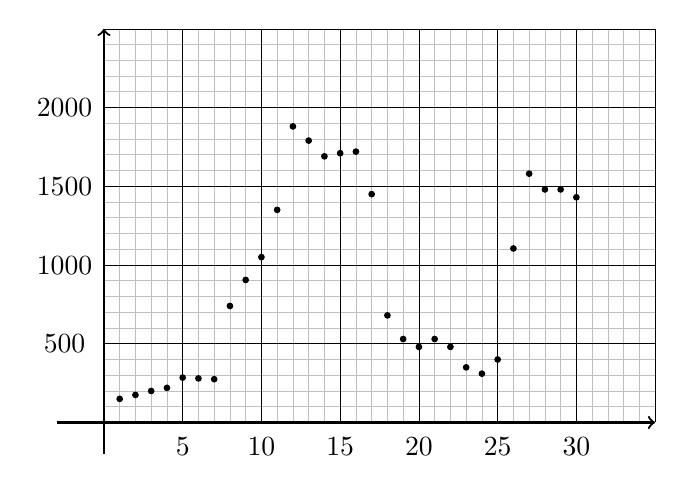
\begin{tikzpicture}
\tikzstyle{ponto}=[circle, minimum size=2pt, inner sep=0, draw=black, fill=black, shift only]
\draw[help lines,xstep=.2,ystep=.2, lightgray] (0,0) grid (7,5);
\draw[help lines, black, xstep=1, ystep=1] (0,0) grid (7,5);
\draw[thick,->](-.6,0)--(7,0);
\draw[thick,->](0,-.4)--(0,5);
\foreach \x in {5, 10, ..., 30}
\draw(.2*\x,-.3)node{\x};
\foreach \y in {500, 1000, 1500, 2000}
\draw(-.5, .002*\y)node{\y};
\node [ponto] at (.2,.3){};
\node [ponto] at (.4,.35){};\node [ponto] at (.6,.4){};\node [ponto] at (.8,.44){};   \node [ponto] at (1,.57){};\node [ponto] at (1.2,.56){};\node [ponto] at (1.4,.55){};\node [ponto] at (1.6,1.48){};\node [ponto] at (1.8,1.81){};\node [ponto] at (2,2.1){};\node [ponto] at (2.2,2.7){};\node [ponto] at (2.4,3.76){};\node [ponto] at (2.6,3.58){};\node [ponto] at (2.8,3.38){};\node [ponto] at (3,3.42){};\node [ponto] at (3.2,3.44){};\node [ponto] at (3.4,2.9){};\node [ponto] at (3.6,1.36){};\node [ponto] at (3.8,1.06){};\node [ponto] at (4,.96){};\node [ponto] at (4.2,1.06){};\node [ponto] at (4.4,.96){};\node [ponto] at (4.6,.7){};\node [ponto] at (4.8,.62){};\node [ponto] at (5.,.8){};\node [ponto] at (5.2,2.21){};\node [ponto] at (5.4,3.16){};\node [ponto] at (5.6,2.96){};;  \node [ponto] at (5.8,2.96){};;\node [ponto] at (6,2.86){};
\end{tikzpicture}
\end{figure}
\begin{enumerate}
\item {} 
Quantas vezes a \emph{hashtag} foi mencionada mais de 1500 vezes em um dia?

\item {} 
Em que dia a \emph{hashtag} foi mais citada?

\item {} 
Identifique todos os períodos em que houve crescimento no número de citações.

\item {} 
Faça o mesmo para o decrescimento.

\item {} 
Escreva um parágrafo explicando o comportamento global do gráfico, apontando possíveis causas para as variações observadas.

\end{enumerate}



\ifdefined\prof
\begin{solucao}
\begin{enumerate}

\item $6$ vezes.

\item No décimo segundo dia.

\item Do segundo ao sexto dia, do sétimo ao décimo segundo dia, do décimo quarto ao décimo sexto dia, entre o vigésimo e vigésimo primeiro dia e entre o vigésimo quarto e vigésimo sétimo dia.

\item Do primeiro para o segundo dia, do sexto para o sétimo dia, do décimo segundo ao décimo quarto dia, do décimo sexto ao vigésimo dia e entre o vigésimo primeiro ao vigésimo quarto dia.

\item Resposta variada.

\end{enumerate}
\end{solucao}
\fi

\end{document}